\section{CFPQ Full-Stack Support}

In order to provide full-stack support of CFPQ it is necessatry to choose an appropriatr graph database.
It was shown by Arseniy Terekhov et al. in~\cite{10.1145/3398682.3399163} that matrix-based algorithm can be naturally integrated into RedisGraph graph database because both, the algorithm and the database, operates over matrix representation of graphs.
Moreover, RedisGraph supports Cypher as a query language and there is a proposal which describes Cypher extension which allows one to specify context-free constraints.
Thus we choose RedisGraph as a base for our solution.  


\subsection{Cypher Extending}
\label{subsec:cypher-extension}

The first what we should do is to extend Cypher to be able to express context-free constraints.
There is a description of the respective Cypher syntax extension\footnote{\label{cypher-proposal}Formal syntax specification: \url{https://github.com/thobe/openCypher/blob/rpq/cip/1.accepted/CIP2017-02-06-Path-Patterns.adoc\#11-syntax}. Access date: 19.07.2020.}, proposed by Tobias Lindaaker, but this syntax does not implement yet in Cypher parsers.

This extension introduces path patterns, which are a more powerful alternative to relationship patterns. Path patterns allow you to express regular constrains over basic patterns such as relationship and node patterns. Just like relationship patterns they can be specified in the MATCH clause between the node patterns.

\begin{algorithm}
\floatname{algorithm}{Listing}
\begin{algorithmic}[1]
\caption{Example of using a simple path pattern}
\label{lst:cypher-example-1}
\State MATCH (v)-/ [:A (:X) :B] | [:C (:Y) :D] /->(to)
\State RETURN v, to
\end{algorithmic}
\end{algorithm}

The listing~\ref{lst:cypher-example-1} provides an example of query in extended syntax with a simple path pattern. In this example there are relationship patterns :A, :B, :C :D and node patterns (:X), (:Y). The square brackets are used for grouping parts of the pattern. The $|$ symbol denotes alternative between corresponding paths and the whitespace denotes sequence of paths. So the result of executing the query on the graph $D$ will be the following set of vertex pairs:
\begin{align*}
\{(v, to): \exists \pi = (v,r_1,u,r_2,to) \in Paths(D):& \\
\begin{sqcases}
    t(r_1) = A, l(u) = X, t(r_2) = B  \\
    t(r_1) = C, l(u) = Y, l(r_2) = D
\end{sqcases}&\}
\end{align*}

Main feature which allows one to specify context-free constraints is a \textit{named path patterns}: one can specify a name for path pattern and after that use it in other patterns, or in the same pattern. Using this feature, structure of query is pretty similar to context-free grammar in the Extended Backus–Naur Form.

\begin{algorithm}
\floatname{algorithm}{Listing}
\begin{algorithmic}[1]
\caption{Example of using a named path pattern}
\label{lst:cypher-example-2}
\State PATH PATTERN S = ()-/ [:A $\sim$S :B] | [:A :B] /->()
\State MATCH (v)-/ $\sim$S /->(to)
\State RETURN v, to
\end{algorithmic}
\end{algorithm}

The listing~\ref{lst:cypher-example-2} shows an example of using named path patterns. They can be defined in the PATH PATTERN clause and referenced within any other path pattern. In order to explain the semantics of the query let`s consider contest-free grammar $G=(N, \Sigma, P, S)$ with $N=\{S\}$, $\Sigma=\{A,B\}$ and $P=\{S \xrightarrow{} A B, S \xrightarrow{} ASB \}$. Then $L(G)=\{A^nB^n: n \in \mathbb{N}\}$ specifies restrictions on the path labels and query result on the graph $D$ will be as follows:

\begin{align*}
\{ (v, to): &~\exists \pi=(v,r_1,u_1,...,r_n,to) \in Paths(D): \\
            &t(r_1)t(r_2)...t(r_n) \in L(G) \}
\end{align*}

Thus this Cypher extension allows one express more complex queries including context-free path queries.
RedisGraph database supports subset of Cypher language and uses \texttt{libcypher-parser}\footnote{The \texttt{libcypher-parser} is an open-source parser library for Cypher query language. GitHub repository of the project: \url{https://github.com/cleishm/libcypher-parser}. Access date: 19.07.2020.} library to parse queries.
We extend this library by intoducing new syntax proposed \footnoteref{cypher-proposal}. We implement\footnote{The modified libsypher-pareser library with support of syntax for path patterns: \url{https://github.com/YaccConstructor/libcypher-parser}. Access date: 19.07.2020.} full extension, not only part which is necessary for simple CFPQ. 

\subsection{RedisGraph Intro (TODO: move to introduction)}

Named path patterns described in \autoref{subsec:cypher-extension} allows one to specify context-free constrains on the paths. In order to support the execution of these types of queries we need to extend backend of the RedisGraph database and integrate a suitable CFPQ algorithm into it. 

There are quite a few algorithms that solve CFPQ problem~\ref{...,...,...}, but their running time makes them unsuitable for practical use~\ref{Neo4J-fail}. Recent studies~\ref{NikitaMishin, simpleton} have shown that one can achieve high performance through the use of matrix-based algorithms. These studies were conducted to analyze the performance of the Rustam Azimov algorithm described in \autoref{subsec:rustam-algo} and have shown that it is acceptable for practical application.

Using the Rustam Azimov algorithm one can only find paths between all pairs of vertexes at once and in some cases it is quite wasteful. Queries to graph databases can be specified so that when they are executed, it is required to find paths from a given set of initial vertices. This set can be quite small due to the different filtering specified in the query. For example in the listing~\ref{lst:cypher-example-3} path pattern \colorbox{blue!10}{-/ $\sim$S /->} follows pattern \colorbox{blue!10}{(v)-[r]->(u)}. The WHERE clause specifies some arbitrary predicate \colorbox{blue!10}{p(v, r, u)} which also fixes a set of initial vertexes for a paths that must satisfy path pattern \colorbox{blue!10}{S}. Depending on this predicate, this set of vertexes can have different sizes and for proper practical use the running time of the CFPQ algorithm should be sensitive to this.

\begin{algorithm}
\floatname{algorithm}{Listing}
\begin{algorithmic}[1]
\caption{...}
\label{lst:cypher-example-3}
\State PATH PATTERN S = ()-/ :A [$\sim$S | ()] :B /->()
\State MATCH (v)-[r]->(u)-/ $\sim$S /->(to)
\State WHERE p(v, r, u)
\State RETURN to
\end{algorithmic}
\end{algorithm}

The Multi-Source algorithm described in~\autoref{sec:multi-source-algo} is sensitive to the initial set of vertices and is therefore well suited for graph database query scenarios. In addition, it is based on matrix operations and works with graphs as sparse matrices, so it is suitable for integration in RedisGraph.

\subsection{RedisGraph extension}
This section describes the implementation of support for executing queries with the extended syntax in the RedisGraph. Throughout this section, we consider executing the example query from listing~\autoref{lst:cypher-example-3} for the graph from~\autoref{fig:example_input_graph}. $\mathcal{M}$ and $\mathcal{N}$ denotes adjacency and vertex label matrices of $G$ respectively. 

\begin{algorithm}
\floatname{algorithm}{Listing}
\begin{algorithmic}[1]
\caption{Query with path patterns example}
\label{lst:cypher-example-3}
\State PATH PATTERN S = ()-/ [:C $\sim$S :D] | [:C (:Y) :D] /->()
\State MATCH (v:X)-[:A]->()-/ :B $\sim$S /->(to)
\State RETURN v, to
\end{algorithmic}
\end{algorithm}

\subsubsection{Execution plan building}
\begin{figure}[h]
  \centering
  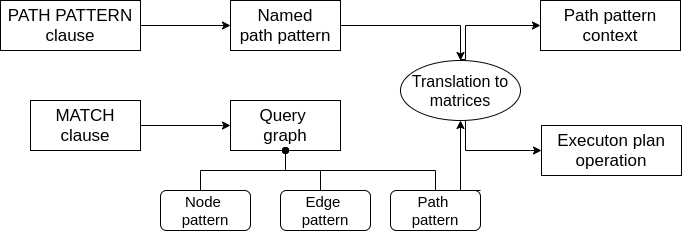
\includegraphics[width=\linewidth]{execution-plan-building.png}
  \caption{Extension diagram for building a query execution plan}
  \label{fig:execution-plan-construction}
\end{figure}

In the RedisGraph the main part of processing a query is building its execution plan. Execution plan consists of operations that perform basic processing such as filtering, pattern matching, aggregation and result construction. The diagram of its construction !!! is shown in~\autoref{fig:execution-plan-construction}. It can be divided into two parts --- processing named and unnamed path patterns, which are described below.

Let`s consider the part that associated with unnamed path patterns. Unnamed path patterns relates to the pattern matching operations and is very similar to relationship patterns from the original Cypher. All pattern matching operations are derived from the MATCH clause that consists of relationship patterns and node patterns. In the example query there is a relationship pattern $r = $\textit{-[:A]->}, path pattern $p$ = \textit{-/ :B ~S /->} and node pattern $n = $\textit{(:X)}. In the first stage of processing, these patterns turn into an intermediate representation --- the \textit{query graph}. The nodes and edges of the query graph corresponds to node and relationship patterns. We extended query graph to be able to contain path patterns. Thus the query graph edges can be either relationship or path patterns, which are stored in a more convenient intermediate representation other than AST. The query graph for patterns $p, r$ and $n$ is shown in~\autoref{fig:query_graph}.

\begin{figure}[h]
    \centering        
    \begin{tikzpicture}[shorten >=0.5pt,auto]
       \node[state] (q_0)                        {$n$};
       \node[state] (q_1) [right=of q_0]         {};
       \node[state] (q_2) [right=of q_1]         {};
        \path[->]
        (q_0) edge  node {$r$} (q_1)
        (q_1) edge  node {$p$} (q_2);
    \end{tikzpicture}
    \caption{The example of input graph $\mathcal{G}$}
    \label{fig:query_graph}
\end{figure}

At the second stage, the query graph is translated into algebraic expressions over matrices. The abstract syntax of an algebraic expression is provided in~\autoref{fig:alg-expr}. Thus the algebraic expression is an expression with addition, multiplication and transposition operations whose operands are matrices. To support references to named paths patterns in algebraic expressions we added a matrix operand \lstinline{Ref(ref)} that stores a reference. In order to translate the query graph RedisGraph first linearizes it and then splits it into small paths. To support path patterns we extended the split processing so that each path pattern corresponds to exactly one path after query graph splitting. For example the query graph in~\autoref{fig:query_graph} is very simple and is divided into three patterns $n, r$ and $p$. After that, each path is translated into a single algebraic expression. We developed the semantics of path patterns in terms of algebraic expressions and implemented translation. For example node pattern $n$ translates to $AlgExp(n) = \mathcal{N}^X$, relationship pattern $r$ to $AlgExp(r) = \mathcal{M}^A$ and path pattern $p$ to $AlgExp(p) = \mathcal{M}^B * Ref(S)$.

% For example the query graph in .

\begin{figure}[H]
\caption{Algebraic expression abstract syntax}
\label{fig:alg-expr}
\begin{align*}
\begin{split}
AlgExpr= ~ &(AlgExpr + AlgExpr)~| \\
           &(AlgExpr * AlgExpr)~| \\
           &Transpose(AlgExpr)~| \\
           &Matrix~| \\
           &Ref(ref)        
\end{split}
\end{align*}
\end{figure}

After obtaining algebraic expressions they are used to construct execution plan operations. Each operation is derived from a single algebraic expression that is involved in the further execution of the corresponding operation. For example for the $AlgExp(r)$ and $AlgExp(n)$ will be created \textit{CondTraverse(AlgExp(r))} and \textit{LabelScan(AlgExp(n))} operations respectively which already existed in RedisGraph. For expressions that correspond to path patterns we created a new \textit{CFPQTraverse} operation. Thus algebraic expression of pattern $p$ will be stored in the new \textit{CFPQTraverse}(AlgExp(p)) operation. During the query execution this operation performs path pattern matching and solves context-free path reachability problem if necessary. This completes the part of the query execution plan building which concerns unnamed path patterns.

Another processing that occurs during the execution plan construction and was supported by us is related to named path patterns. They are processed independently of the unnamed path patterns found in MATCH clause and don't produce execution plan operations. 

All named path patterns are collected from \lstinline{PATH PATTERN} clauses. In the example query there is a path pattern \textit{S = ()-/ [:C $\sim$S :D] | [:C (:Y) :D] /->()}. Then this named path patterns translated into algebraic expressions and stored in the corresponding global context of the query --- \textit{path pattern context}. This storage provides mapping between the path pattern name and its algebraic expression and can be used both when building an execution plan and during its execution. For the example query it will be as follows:

$$\{ S \xrightarrow{} \mathcal{M}^C * Ref(S) * \mathcal{M}^D + \mathcal{M}^C * \mathcal{N}^Y * \mathcal{M}^D \}$$

Thus after execution plan building we receive \textit{CFPQTraverse} operations that correspond to unnamed path patterns in MATCH clause and \textit{path pattern context} that stores all named path patterns from \lstinline{PATH PATTERN} clauses. Therefore we can proceed to the stage of execution plan evaluation.


\subsubsection{Execution plan evaluating}
\label{subsubsec:execution-plan-evaluating}

\begin{figure}[h!]
  \centering
  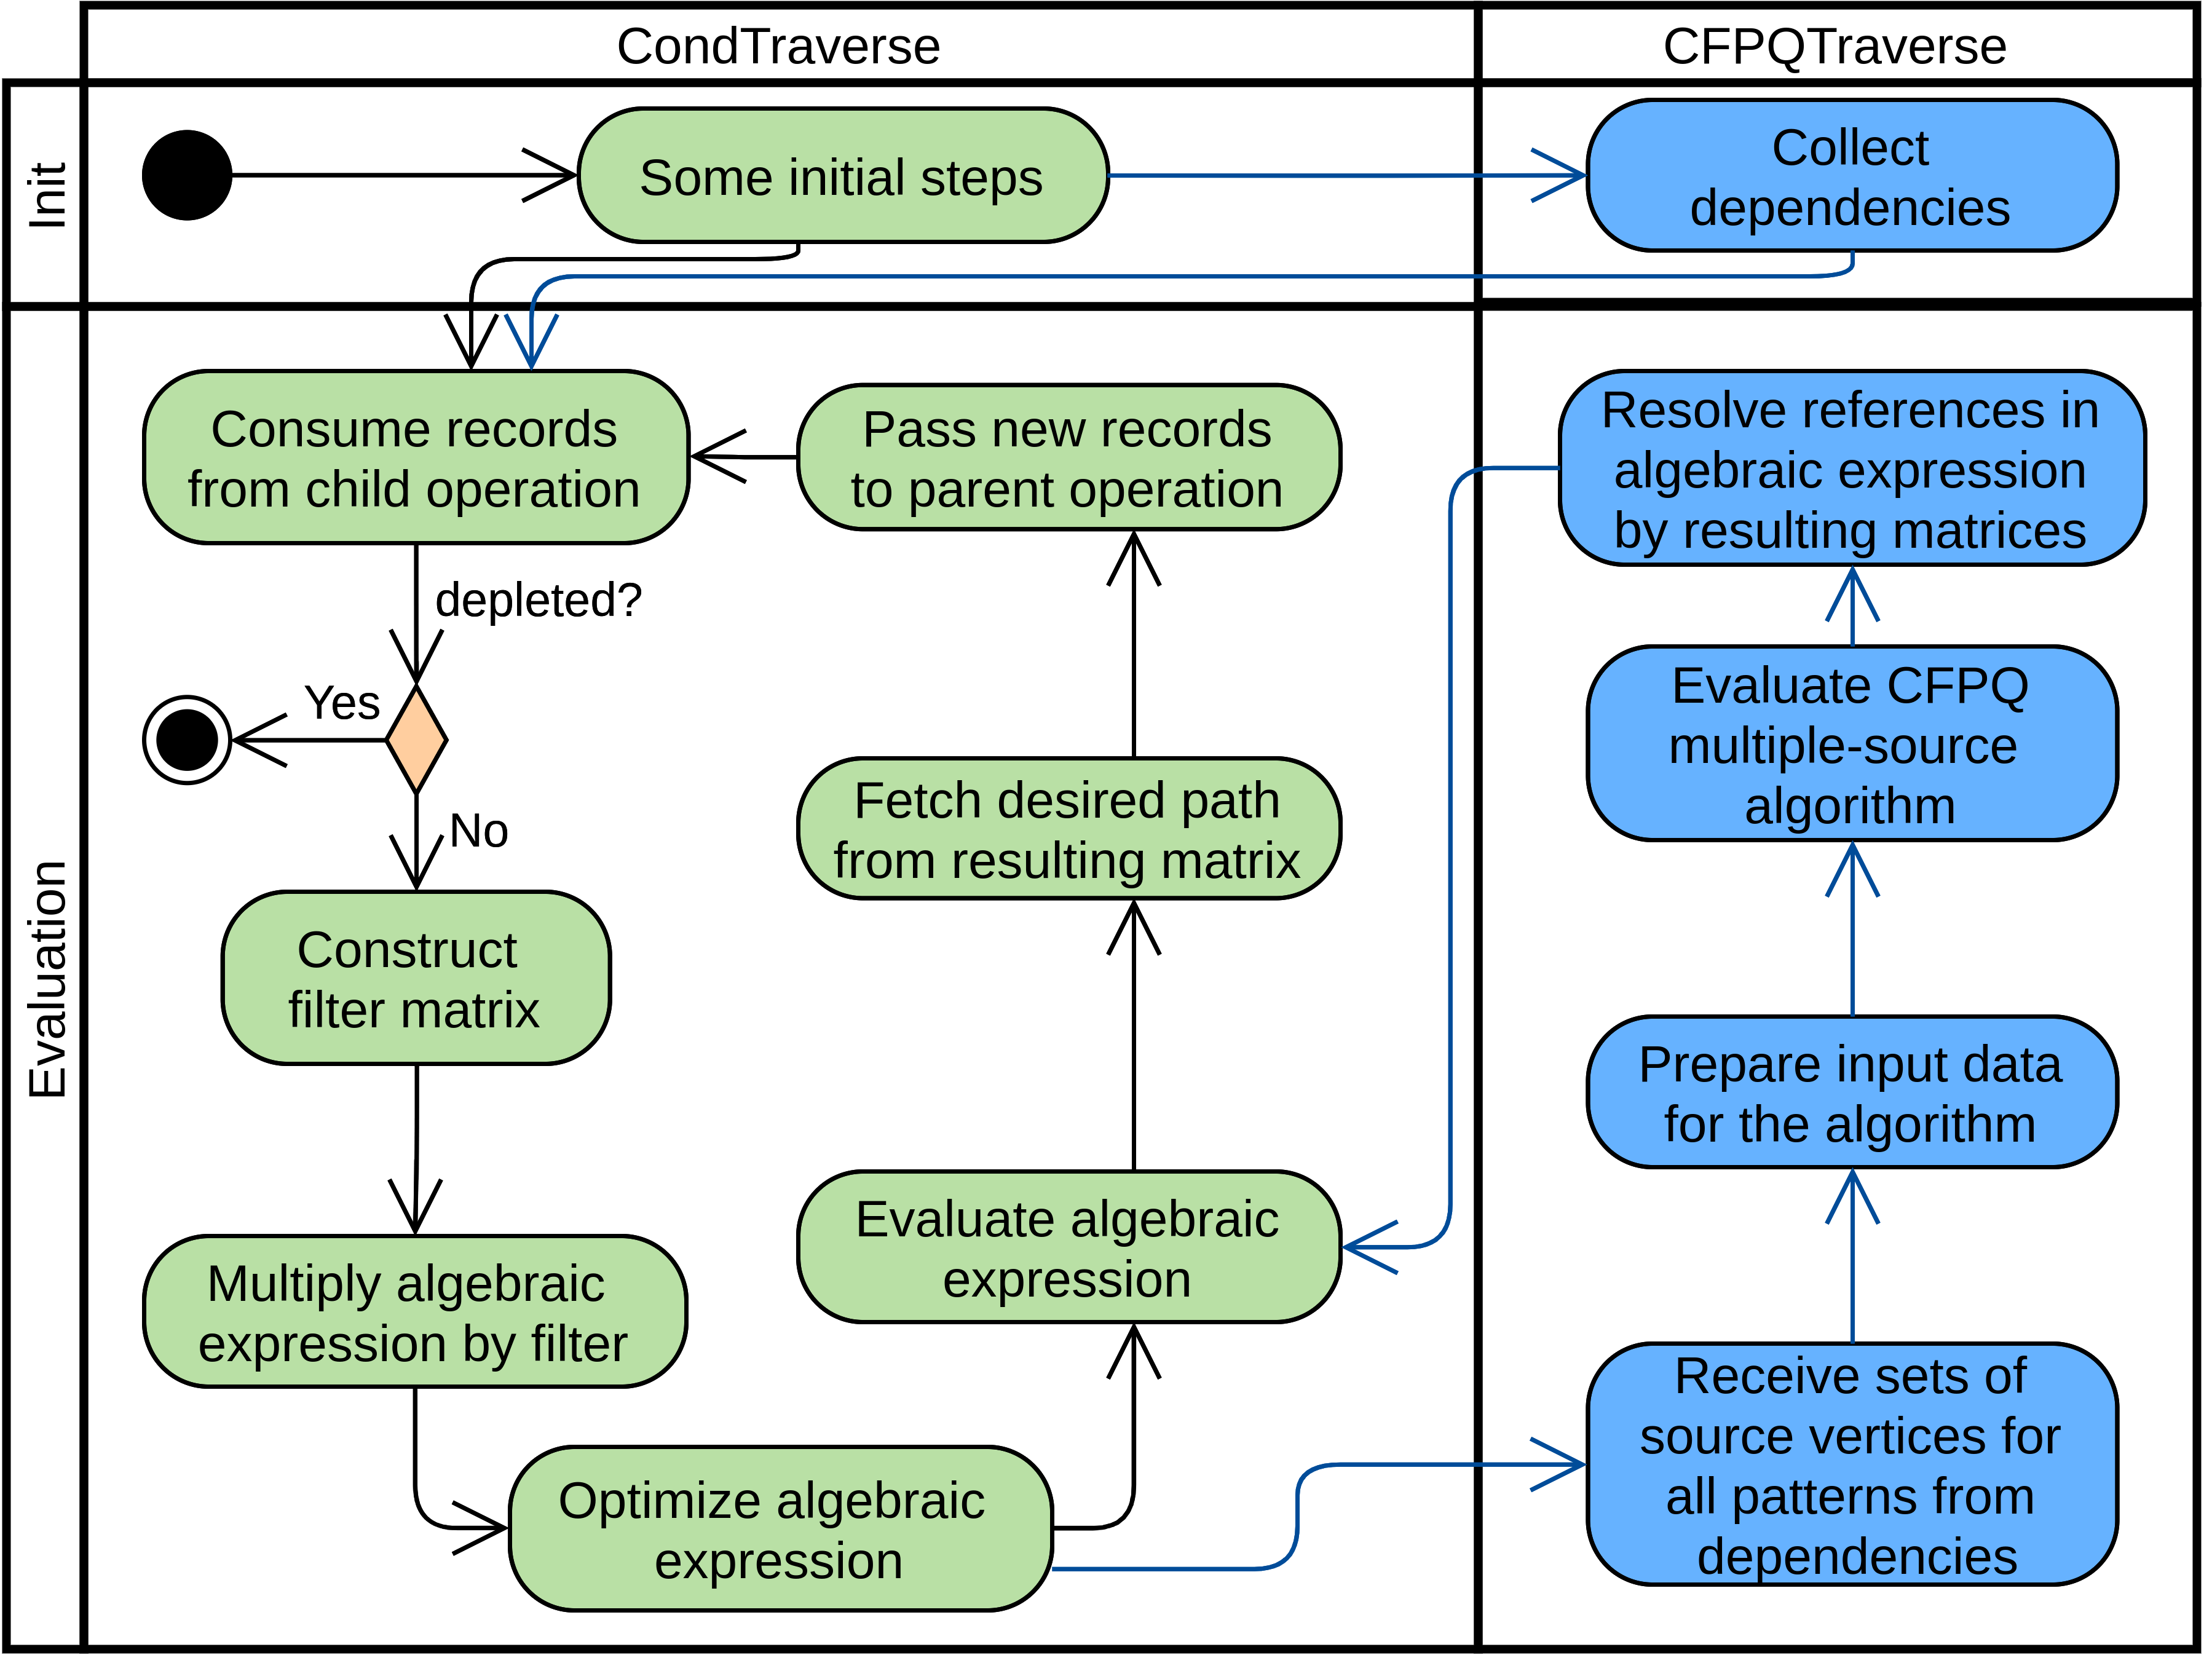
\includegraphics[width=\linewidth]{pictures/execution-plan-evaluation.png}
  \caption{CFPQTraverse and CondTraverse evaluation}
  \label{fig:execution-plan-evaluation}
\end{figure}

The remaining part of query processing is evaluation its execution plan. This section describes how the \lstinline{CFPQTraverse} operation is performed. For explanation, we use example graph $G$ from~\autoref{fig:example_input_graph} and execution plan operations $LabelScan(n)$, $CondTraverse(r)$ and $CfpqTraverse(p)$ that were obtained in the chapter for example query.

Let`s first consider the structure of the execution plan operations. Operations have parent-child relationships, so they are formed into a tree. For example, the part of execution plan that derived from example query is shown in~\autoref{fig:execution-plan-operations}. Each operation can consume a record from a child operation, process it and produce another one for the parent. Records contain information necessary for the parent operation, as well as everything to restore the response, such as identifiers of accumulated vertices and edges.

\begin{figure}[h]
    \centering        
    \begin{tikzpicture}[shorten >=0.5pt,auto]
       \node (q_0) [draw,thick,minimum width=2cm,minimum height=0.5cm]                        {LabelScan(AlgExp(n))};
       \node (q_1) [draw,thick,minimum width=2cm,minimum height=0.5cm, above=of q_0]                        {CondTraverse(AlgExp(r))};
        \node (q_2) [draw,thick,minimum width=2cm,minimum height=0.5cm, right=of q_1]                        {CFPQTraverse(AlgExp(p))};
        \path[->]
        (q_0) edge[bend left, left]  node {produce} (q_1)
        (q_1) edge[bend left, right] node {consume} (q_0)
        (q_1) edge[bend left, above] node {produce} (q_2)
        (q_2) edge[bend left, above] node {consume} (q_1);
    \end{tikzpicture}
    \caption{Example of part of the execution plan}
    \label{fig:execution-plan-operations}
\end{figure}

The \lstinline{CFPQTraverse} operation is based on \lstinline{CondTraverse} operation that already exists in the RedisGraph and performs a patterns matching. The activity diagram of this operations is shown in~\autoref{fig:execution-plan-evaluation} and described below. Actions that corresponds to \lstinline{CondTraverse} operation are highlighted in green, actions of the \lstinline{CFPQTraverse} operation that extend \lstinline{CondTraverse} are highlighted in blue.

The \lstinline{CondTraverse} works as follows. At first it consumes several records from the child operation and accumulates them in the buffer. Here each record corresponds to the path that built by the child operation. For simplicity we can presume that each record is the destination vertex of the path. For example for the graph $G$ the \textit{CondTraverse} from~\autoref{fig:execution-plan-operations} make \textit{LabelScan} operation to produce vertices with the label $X$ and then store the resulting set of vertices $\{1, 3\}$ in the buffer. The task of the \lstinline{CondTraverse} is to continue the path from this vertices in such way that the resulting path satisfies pattern corresponding to this operation. To do this \lstinline{CondTraverse} uses the algebraic expression obtained in the previous step. The resulting matrix of this expression represents all pairs of vertices between which there is a path satisfying the pattern. In order to find paths that start from given sources vertices \lstinline{CondTraverse} uses a filter matrix. This matrix is constructed from the destination vertices retrieved from the record buffer and resembles matrix from boolean decomposition of label vertex matrix. For example filter matrix of set $\{1, 3\}$ is $ r_{f}=\{(1, 1), (3, 3)\}$. Then this matrix is multiplied to the right by \textit{AlgExp(r) = A} and we get algebraic expression $r_{f} * A$. Only after that this expression is evaluated and we get the matrix $\{(1, 2)\}$. This matrix exactly corresponds to all paths of length one where the source vertex is labelled by X and the edge is labeled by A. Then this paths are passed to the parent operation, in our case to $CFPQTraverse$, by producing new records.

The \lstinline{CFPQTraverse} operation is arranged in the same way as \lstinline{CondTraverse} but performs some additional work. Since each \lstinline{CFPQTraverse} corresponds to path pattern, its algebraic expression may contain references to named path patterns. Therefore all named path patterns that the algebraic expression depends on must be processed. For this they are extracted from \textit{path pattern context} and stored in the \textit{set of operation dependencies} during its initialization. In this case, dependencies are extracted recursively, so that references inside named path patterns are also extracted.

The \lstinline{CFPQTraverse} execution stage starts the same way as \lstinline{CondTraverse}. First filter matrix is constructed from record buffer and embedded in the algebraic expression. Then for each reference we need to determinate the set of source vertices. This can be done during algebraic expression evaluation which we extended for this purpose. After that we have everything to run \textit{multiple-source} CFPQ algorithm to resolve all dependencies. This algorithm is slightly different from the one described in~\autoref{sec:multiple-source-algo} and is a generalization of it. It receives the \textit{set of operation dependencies} and sets of source vertices. After running this algorithm a matrix is obtained for each named path pattern. This matrices represent a set of pairs of vertices between which there is a path that satisfies the pattern. Then all references in the algebraic expression are replaced with the resulting matrices and the algebraic expression is evaluated. Finally as well as \lstinline{CondTraverse}, \lstinline{CFPQTraverse} extracts desired paths from resulting matrix and passes them to parent operation.

% the \lstinline{CFPQTraverse} executes \textit{multiple-source} algorithm to resolve context-free reachability problem.

% CFPQ to matrix expressions, etc. General schema of integration. Limits, restrictions, examples, etc.

\subsection{Evaluation}

Small basic evalustion on real-world graph (geo?).
In order to show, that performance is reasonable.

Regular quries. Comparison with other DB?

